\documentclass[1p]{elsarticle_modified}
%\bibliographystyle{elsarticle-num}

%\usepackage[colorlinks]{hyperref}
%\usepackage{abbrmath_seonhwa} %\Abb, \Ascr, \Acal ,\Abf, \Afrak
\usepackage{amsfonts}
\usepackage{amssymb}
\usepackage{amsmath}
\usepackage{amsthm}
\usepackage{scalefnt}
\usepackage{amsbsy}
\usepackage{kotex}
\usepackage{caption}
\usepackage{subfig}
\usepackage{color}
\usepackage{graphicx}
\usepackage{xcolor} %% white, black, red, green, blue, cyan, magenta, yellow
\usepackage{float}
\usepackage{setspace}
\usepackage{hyperref}

\usepackage{tikz}
\usetikzlibrary{arrows}

\usepackage{multirow}
\usepackage{array} % fixed length table
\usepackage{hhline}

%%%%%%%%%%%%%%%%%%%%%
\makeatletter
\renewcommand*\env@matrix[1][\arraystretch]{%
	\edef\arraystretch{#1}%
	\hskip -\arraycolsep
	\let\@ifnextchar\new@ifnextchar
	\array{*\c@MaxMatrixCols c}}
\makeatother %https://tex.stackexchange.com/questions/14071/how-can-i-increase-the-line-spacing-in-a-matrix
%%%%%%%%%%%%%%%

\usepackage[normalem]{ulem}

\newcommand{\msout}[1]{\ifmmode\text{\sout{\ensuremath{#1}}}\else\sout{#1}\fi}
%SOURCE: \msout is \stkout macro in https://tex.stackexchange.com/questions/20609/strikeout-in-math-mode

\newcommand{\cancel}[1]{
	\ifmmode
	{\color{red}\msout{#1}}
	\else
	{\color{red}\sout{#1}}
	\fi
}

\newcommand{\add}[1]{
	{\color{blue}\uwave{#1}}
}

\newcommand{\replace}[2]{
	\ifmmode
	{\color{red}\msout{#1}}{\color{blue}\uwave{#2}}
	\else
	{\color{red}\sout{#1}}{\color{blue}\uwave{#2}}
	\fi
}

\newcommand{\Sol}{\mathcal{S}} %segment
\newcommand{\D}{D} %diagram
\newcommand{\A}{\mathcal{A}} %arc


%%%%%%%%%%%%%%%%%%%%%%%%%%%%%5 test

\def\sl{\operatorname{\textup{SL}}(2,\Cbb)}
\def\psl{\operatorname{\textup{PSL}}(2,\Cbb)}
\def\quan{\mkern 1mu \triangleright \mkern 1mu}

\theoremstyle{definition}
\newtheorem{thm}{Theorem}[section]
\newtheorem{prop}[thm]{Proposition}
\newtheorem{lem}[thm]{Lemma}
\newtheorem{ques}[thm]{Question}
\newtheorem{cor}[thm]{Corollary}
\newtheorem{defn}[thm]{Definition}
\newtheorem{exam}[thm]{Example}
\newtheorem{rmk}[thm]{Remark}
\newtheorem{alg}[thm]{Algorithm}

\newcommand{\I}{\sqrt{-1}}
\begin{document}

%\begin{frontmatter}
%
%\title{Boundary parabolic representations of knots up to 8 crossings}
%
%%% Group authors per affiliation:
%\author{Yunhi Cho} 
%\address{Department of Mathematics, University of Seoul, Seoul, Korea}
%\ead{yhcho@uos.ac.kr}
%
%
%\author{Seonhwa Kim} %\fnref{s_kim}}
%\address{Center for Geometry and Physics, Institute for Basic Science, Pohang, 37673, Korea}
%\ead{ryeona17@ibs.re.kr}
%
%\author{Hyuk Kim}
%\address{Department of Mathematical Sciences, Seoul National University, Seoul 08826, Korea}
%\ead{hyukkim@snu.ac.kr}
%
%\author{Seokbeom Yoon}
%\address{Department of Mathematical Sciences, Seoul National University, Seoul, 08826,  Korea}
%\ead{sbyoon15@snu.ac.kr}
%
%\begin{abstract}
%We find all boundary parabolic representation of knots up to 8 crossings.
%
%\end{abstract}
%\begin{keyword}
%    \MSC[2010] 57M25 
%\end{keyword}
%
%\end{frontmatter}

%\linenumbers
%\tableofcontents
%
\newcommand\colored[1]{\textcolor{white}{\rule[-0.35ex]{0.8em}{1.4ex}}\kern-0.8em\color{red} #1}%
%\newcommand\colored[1]{\textcolor{white}{ #1}\kern-2.17ex	\textcolor{white}{ #1}\kern-1.81ex	\textcolor{white}{ #1}\kern-2.15ex\color{red}#1	}

{\Large $\underline{12n_{0435}~(K12n_{0435})}$}

\setlength{\tabcolsep}{10pt}
\renewcommand{\arraystretch}{1.6}
\vspace{1cm}\begin{tabular}{m{100pt}>{\centering\arraybackslash}m{274pt}}
\multirow{5}{120pt}{
	\centering
	\includegraphics[width=112pt]{../../../GIT/diagram.site/Diagrams/png/2524_12n_0435.png}\\
\ \ \ A knot diagram\footnotemark}&
\allowdisplaybreaks
\textbf{Linearized knot diagam} \\
\cline{2-2}
 &
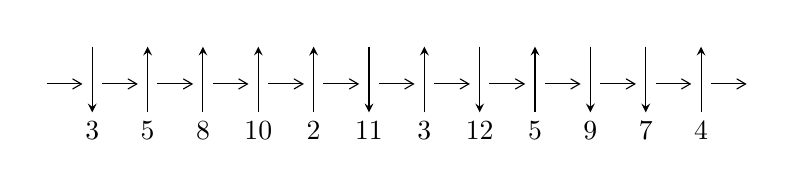
\begin{tikzpicture}[x=20pt, y=17pt]
	% nodes
	\node (C0) at (0, 0) {};
	\node (C1) at (1, 0) {};
	\node (C1U) at (1, +1) {};
	\node (C1D) at (1, -1) {3};

	\node (C2) at (2, 0) {};
	\node (C2U) at (2, +1) {};
	\node (C2D) at (2, -1) {5};

	\node (C3) at (3, 0) {};
	\node (C3U) at (3, +1) {};
	\node (C3D) at (3, -1) {8};

	\node (C4) at (4, 0) {};
	\node (C4U) at (4, +1) {};
	\node (C4D) at (4, -1) {10};

	\node (C5) at (5, 0) {};
	\node (C5U) at (5, +1) {};
	\node (C5D) at (5, -1) {2};

	\node (C6) at (6, 0) {};
	\node (C6U) at (6, +1) {};
	\node (C6D) at (6, -1) {11};

	\node (C7) at (7, 0) {};
	\node (C7U) at (7, +1) {};
	\node (C7D) at (7, -1) {3};

	\node (C8) at (8, 0) {};
	\node (C8U) at (8, +1) {};
	\node (C8D) at (8, -1) {12};

	\node (C9) at (9, 0) {};
	\node (C9U) at (9, +1) {};
	\node (C9D) at (9, -1) {5};

	\node (C10) at (10, 0) {};
	\node (C10U) at (10, +1) {};
	\node (C10D) at (10, -1) {9};

	\node (C11) at (11, 0) {};
	\node (C11U) at (11, +1) {};
	\node (C11D) at (11, -1) {7};

	\node (C12) at (12, 0) {};
	\node (C12U) at (12, +1) {};
	\node (C12D) at (12, -1) {4};
	\node (C13) at (13, 0) {};

	% arrows
	\draw[->,>={angle 60}]
	(C0) edge (C1) (C1) edge (C2) (C2) edge (C3) (C3) edge (C4) (C4) edge (C5) (C5) edge (C6) (C6) edge (C7) (C7) edge (C8) (C8) edge (C9) (C9) edge (C10) (C10) edge (C11) (C11) edge (C12) (C12) edge (C13) ;	\draw[->,>=stealth]
	(C1U) edge (C1D) (C2D) edge (C2U) (C3D) edge (C3U) (C4D) edge (C4U) (C5D) edge (C5U) (C6U) edge (C6D) (C7D) edge (C7U) (C8U) edge (C8D) (C9D) edge (C9U) (C10U) edge (C10D) (C11U) edge (C11D) (C12D) edge (C12U) ;
	\end{tikzpicture} \\
\hhline{~~} \\& 
\textbf{Solving Sequence} \\ \cline{2-2} 
 &
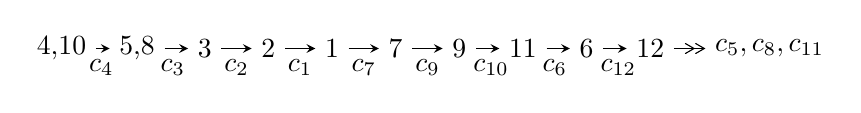
\begin{tikzpicture}[x=23pt, y=7pt]
	% node
	\node (A0) at (-1/8, 0) {4,10};
	\node (A1) at (17/16, 0) {5,8};
	\node (A2) at (17/8, 0) {3};
	\node (A3) at (25/8, 0) {2};
	\node (A4) at (33/8, 0) {1};
	\node (A5) at (41/8, 0) {7};
	\node (A6) at (49/8, 0) {9};
	\node (A7) at (57/8, 0) {11};
	\node (A8) at (65/8, 0) {6};
	\node (A9) at (73/8, 0) {12};
	\node (C1) at (1/2, -1) {$c_{4}$};
	\node (C2) at (13/8, -1) {$c_{3}$};
	\node (C3) at (21/8, -1) {$c_{2}$};
	\node (C4) at (29/8, -1) {$c_{1}$};
	\node (C5) at (37/8, -1) {$c_{7}$};
	\node (C6) at (45/8, -1) {$c_{9}$};
	\node (C7) at (53/8, -1) {$c_{10}$};
	\node (C8) at (61/8, -1) {$c_{6}$};
	\node (C9) at (69/8, -1) {$c_{12}$};
	\node (A10) at (11, 0) {$c_{5},c_{8},c_{11}$};

	% edge
	\draw[->,>=stealth]	
	(A0) edge (A1) (A1) edge (A2) (A2) edge (A3) (A3) edge (A4) (A4) edge (A5) (A5) edge (A6) (A6) edge (A7) (A7) edge (A8) (A8) edge (A9) ;
	\draw[->>,>={angle 60}]	
	(A9) edge (A10);
\end{tikzpicture} \\ 

\end{tabular} \\

\footnotetext{
The image of knot diagram is generated by the software ``\textbf{Draw programme}" developed by Andrew Bartholomew(\url{http://www.layer8.co.uk/maths/draw/index.htm\#Running-draw}), where we modified some parts for our purpose(\url{https://github.com/CATsTAILs/LinksPainter}).
}\phantom \\ \newline 
\centering \textbf{Ideals for irreducible components\footnotemark of $X_{\text{par}}$} 
 
\begin{align*}
I^u_{1}&=\langle 
-1.59109\times10^{70} u^{47}+3.54965\times10^{69} u^{46}+\cdots+6.67625\times10^{70} b-1.64708\times10^{71},\\
\phantom{I^u_{1}}&\phantom{= \langle  }1.45455\times10^{70} u^{47}+1.03237\times10^{71} u^{46}+\cdots+1.93611\times10^{72} a-2.56576\times10^{72},\;u^{48}+18 u^{46}+\cdots+13 u+1\rangle \\
I^u_{2}&=\langle 
-2 u^{18}+2 u^{17}+\cdots+b-6,\;-3 u^{19}+4 u^{18}+\cdots+a+6,\;u^{20}- u^{19}+\cdots- u+1\rangle \\
\\
\end{align*}
\raggedright * 2 irreducible components of $\dim_{\mathbb{C}}=0$, with total 68 representations.\\
\footnotetext{All coefficients of polynomials are rational numbers. But the coefficients are sometimes approximated in decimal forms when there is not enough margin.}
\newpage
\renewcommand{\arraystretch}{1}
\centering \section*{I. $I^u_{1}= \langle -1.59\times10^{70} u^{47}+3.55\times10^{69} u^{46}+\cdots+6.68\times10^{70} b-1.65\times10^{71},\;1.45\times10^{70} u^{47}+1.03\times10^{71} u^{46}+\cdots+1.94\times10^{72} a-2.57\times10^{72},\;u^{48}+18 u^{46}+\cdots+13 u+1 \rangle$}
\flushleft \textbf{(i) Arc colorings}\\
\begin{tabular}{m{7pt} m{180pt} m{7pt} m{180pt} }
\flushright $a_{4}=$&$\begin{pmatrix}1\\0\end{pmatrix}$ \\
\flushright $a_{10}=$&$\begin{pmatrix}0\\u\end{pmatrix}$ \\
\flushright $a_{5}=$&$\begin{pmatrix}1\\- u^2\end{pmatrix}$ \\
\flushright $a_{8}=$&$\begin{pmatrix}-0.00751276 u^{47}-0.0533219 u^{46}+\cdots-12.6223 u+1.32521\\0.238322 u^{47}-0.0531683 u^{46}+\cdots+12.7021 u+2.46708\end{pmatrix}$ \\
\flushright $a_{3}=$&$\begin{pmatrix}0.553394 u^{47}-0.134182 u^{46}+\cdots+21.9136 u+6.68234\\0.355711 u^{47}-0.0573944 u^{46}+\cdots+21.1330 u+2.83673\end{pmatrix}$ \\
\flushright $a_{2}=$&$\begin{pmatrix}0.171681 u^{47}-0.0635417 u^{46}+\cdots-0.410390 u+3.71143\\0.377230 u^{47}-0.0534903 u^{46}+\cdots+21.6696 u+2.90737\end{pmatrix}$ \\
\flushright $a_{1}=$&$\begin{pmatrix}-1.01739 u^{47}-0.00588462 u^{46}+\cdots-41.8000 u-8.31915\\-0.575290 u^{47}+0.0697542 u^{46}+\cdots-22.4788 u-3.42421\end{pmatrix}$ \\
\flushright $a_{7}=$&$\begin{pmatrix}-1.22875 u^{47}+0.234716 u^{46}+\cdots-73.9234 u-8.65813\\-0.0478120 u^{47}+0.0300471 u^{46}+\cdots-4.36142 u+1.13699\end{pmatrix}$ \\
\flushright $a_{9}=$&$\begin{pmatrix}- u\\u^3+u\end{pmatrix}$ \\
\flushright $a_{11}=$&$\begin{pmatrix}- u^3\\u^5+u^3+u\end{pmatrix}$ \\
\flushright $a_{6}=$&$\begin{pmatrix}-1.20137 u^{47}+0.213398 u^{46}+\cdots-74.0842 u-8.67754\\0.0502293 u^{47}+0.000898209 u^{46}+\cdots-2.60784 u+1.37666\end{pmatrix}$ \\
\flushright $a_{12}=$&$\begin{pmatrix}-0.442100 u^{47}-0.0756388 u^{46}+\cdots-19.3212 u-4.89494\\-0.575290 u^{47}+0.0697542 u^{46}+\cdots-22.4788 u-3.42421\end{pmatrix}$\\&\end{tabular}
\flushleft \textbf{(ii) Obstruction class $= -1$}\\~\\
\flushleft \textbf{(iii) Cusp Shapes $= -0.724487 u^{47}+0.0435195 u^{46}+\cdots-74.1390 u-1.70909$}\\~\\
\newpage\renewcommand{\arraystretch}{1}
\flushleft \textbf{(iv) u-Polynomials at the component}\newline \\
\begin{tabular}{m{50pt}|m{274pt}}
Crossings & \hspace{64pt}u-Polynomials at each crossing \\
\hline $$\begin{aligned}c_{1}\end{aligned}$$&$\begin{aligned}
&u^{48}+67 u^{47}+\cdots+604670586 u+32137561
\end{aligned}$\\
\hline $$\begin{aligned}c_{2},c_{5}\end{aligned}$$&$\begin{aligned}
&u^{48}+3 u^{47}+\cdots+13144 u+5669
\end{aligned}$\\
\hline $$\begin{aligned}c_{3},c_{7}\end{aligned}$$&$\begin{aligned}
&u^{48}+u^{47}+\cdots+12 u+1
\end{aligned}$\\
\hline $$\begin{aligned}c_{4},c_{9}\end{aligned}$$&$\begin{aligned}
&u^{48}+18 u^{46}+\cdots+13 u+1
\end{aligned}$\\
\hline $$\begin{aligned}c_{6},c_{11}\end{aligned}$$&$\begin{aligned}
&u^{48}+u^{47}+\cdots-2534 u+1167
\end{aligned}$\\
\hline $$\begin{aligned}c_{8}\end{aligned}$$&$\begin{aligned}
&u^{48}-3 u^{47}+\cdots+3 u+1
\end{aligned}$\\
\hline $$\begin{aligned}c_{10}\end{aligned}$$&$\begin{aligned}
&u^{48}+36 u^{47}+\cdots-39 u+1
\end{aligned}$\\
\hline $$\begin{aligned}c_{12}\end{aligned}$$&$\begin{aligned}
&u^{48}+11 u^{47}+\cdots+7155479 u+5008881
\end{aligned}$\\
\hline
\end{tabular}\\~\\
\newpage\renewcommand{\arraystretch}{1}
\flushleft \textbf{(v) Riley Polynomials at the component}\newline \\
\begin{tabular}{m{50pt}|m{274pt}}
Crossings & \hspace{64pt}Riley Polynomials at each crossing \\
\hline $$\begin{aligned}c_{1}\end{aligned}$$&$\begin{aligned}
&y^{48}-157 y^{47}+\cdots+26058532373273318 y+1032822827028721
\end{aligned}$\\
\hline $$\begin{aligned}c_{2},c_{5}\end{aligned}$$&$\begin{aligned}
&y^{48}+67 y^{47}+\cdots+604670586 y+32137561
\end{aligned}$\\
\hline $$\begin{aligned}c_{3},c_{7}\end{aligned}$$&$\begin{aligned}
&y^{48}-9 y^{47}+\cdots-22 y+1
\end{aligned}$\\
\hline $$\begin{aligned}c_{4},c_{9}\end{aligned}$$&$\begin{aligned}
&y^{48}+36 y^{47}+\cdots-39 y+1
\end{aligned}$\\
\hline $$\begin{aligned}c_{6},c_{11}\end{aligned}$$&$\begin{aligned}
&y^{48}-53 y^{47}+\cdots+12171488 y+1361889
\end{aligned}$\\
\hline $$\begin{aligned}c_{8}\end{aligned}$$&$\begin{aligned}
&y^{48}-3 y^{47}+\cdots+33 y+1
\end{aligned}$\\
\hline $$\begin{aligned}c_{10}\end{aligned}$$&$\begin{aligned}
&y^{48}-36 y^{47}+\cdots-575 y+1
\end{aligned}$\\
\hline $$\begin{aligned}c_{12}\end{aligned}$$&$\begin{aligned}
&y^{48}+45 y^{47}+\cdots+12614337897293 y+25088888872161
\end{aligned}$\\
\hline
\end{tabular}\\~\\
\newpage\flushleft \textbf{(vi) Complex Volumes and Cusp Shapes}
$$\begin{array}{c|c|c}  
\text{Solutions to }I^u_{1}& \I (\text{vol} + \sqrt{-1}CS) & \text{Cusp shape}\\
 \hline 
\begin{aligned}
u &= -0.624375 + 0.790739 I \\
a &= \phantom{-}0.652451 + 0.017302 I \\
b &= -0.987977 - 0.377013 I\end{aligned}
 & \phantom{-}3.11335 + 0.59534 I & \phantom{-}8.72046 - 1.05598 I \\ \hline\begin{aligned}
u &= -0.624375 - 0.790739 I \\
a &= \phantom{-}0.652451 - 0.017302 I \\
b &= -0.987977 + 0.377013 I\end{aligned}
 & \phantom{-}3.11335 - 0.59534 I & \phantom{-}8.72046 + 1.05598 I \\ \hline\begin{aligned}
u &= -0.441932 + 0.974715 I \\
a &= -1.49605 - 0.17508 I \\
b &= \phantom{-}0.527184 - 0.376923 I\end{aligned}
 & -3.50502 - 4.85959 I & -3.75126 + 8.82096 I \\ \hline\begin{aligned}
u &= -0.441932 - 0.974715 I \\
a &= -1.49605 + 0.17508 I \\
b &= \phantom{-}0.527184 + 0.376923 I\end{aligned}
 & -3.50502 + 4.85959 I & -3.75126 - 8.82096 I \\ \hline\begin{aligned}
u &= -0.673784 + 0.878510 I \\
a &= -1.13342 - 1.57768 I \\
b &= \phantom{-}1.000680 - 0.446035 I\end{aligned}
 & \phantom{-}2.90064 - 5.69851 I & \phantom{-}8.81108 + 5.67017 I \\ \hline\begin{aligned}
u &= -0.673784 - 0.878510 I \\
a &= -1.13342 + 1.57768 I \\
b &= \phantom{-}1.000680 + 0.446035 I\end{aligned}
 & \phantom{-}2.90064 + 5.69851 I & \phantom{-}8.81108 - 5.67017 I \\ \hline\begin{aligned}
u &= -0.032468 + 0.886041 I \\
a &= \phantom{-}0.75785 + 1.61125 I \\
b &= \phantom{-}0.435941 + 0.357265 I\end{aligned}
 & -1.78883 + 1.42161 I & -2.69512 - 4.63338 I \\ \hline\begin{aligned}
u &= -0.032468 - 0.886041 I \\
a &= \phantom{-}0.75785 - 1.61125 I \\
b &= \phantom{-}0.435941 - 0.357265 I\end{aligned}
 & -1.78883 - 1.42161 I & -2.69512 + 4.63338 I \\ \hline\begin{aligned}
u &= \phantom{-}0.846760 + 0.741793 I \\
a &= \phantom{-}0.152370 - 0.285782 I \\
b &= \phantom{-}0.381842 + 0.020417 I\end{aligned}
 & \phantom{-}0.97742 + 3.01246 I & \phantom{-}6.86160 - 7.48318 I \\ \hline\begin{aligned}
u &= \phantom{-}0.846760 - 0.741793 I \\
a &= \phantom{-}0.152370 + 0.285782 I \\
b &= \phantom{-}0.381842 - 0.020417 I\end{aligned}
 & \phantom{-}0.97742 - 3.01246 I & \phantom{-}6.86160 + 7.48318 I\\
 \hline 
 \end{array}$$\newpage$$\begin{array}{c|c|c}  
\text{Solutions to }I^u_{1}& \I (\text{vol} + \sqrt{-1}CS) & \text{Cusp shape}\\
 \hline 
\begin{aligned}
u &= \phantom{-}0.655494 + 0.992944 I \\
a &= \phantom{-}0.422584 - 0.642594 I \\
b &= -0.135634 - 0.580747 I\end{aligned}
 & \phantom{-}0.46539 + 2.67049 I & \phantom{-}2.00000 - 1.39704 I \\ \hline\begin{aligned}
u &= \phantom{-}0.655494 - 0.992944 I \\
a &= \phantom{-}0.422584 + 0.642594 I \\
b &= -0.135634 + 0.580747 I\end{aligned}
 & \phantom{-}0.46539 - 2.67049 I & \phantom{-}2.00000 + 1.39704 I \\ \hline\begin{aligned}
u &= \phantom{-}0.514823 + 1.094190 I \\
a &= -0.087680 + 0.763881 I \\
b &= \phantom{-}0.882038 + 0.252747 I\end{aligned}
 & -1.61783 + 4.43732 I & \phantom{-}2.00000 - 5.85728 I \\ \hline\begin{aligned}
u &= \phantom{-}0.514823 - 1.094190 I \\
a &= -0.087680 - 0.763881 I \\
b &= \phantom{-}0.882038 - 0.252747 I\end{aligned}
 & -1.61783 - 4.43732 I & \phantom{-}2.00000 + 5.85728 I \\ \hline\begin{aligned}
u &= \phantom{-}1.227510 + 0.143214 I \\
a &= \phantom{-}0.507883 + 0.381592 I \\
b &= -0.99480 + 1.00630 I\end{aligned}
 & -10.62720 + 0.57436 I & \phantom{-0.000000 } 0 \\ \hline\begin{aligned}
u &= \phantom{-}1.227510 - 0.143214 I \\
a &= \phantom{-}0.507883 - 0.381592 I \\
b &= -0.99480 - 1.00630 I\end{aligned}
 & -10.62720 - 0.57436 I & \phantom{-0.000000 } 0 \\ \hline\begin{aligned}
u &= \phantom{-}0.058897 + 1.244960 I \\
a &= \phantom{-}0.47320 - 1.49785 I \\
b &= -1.064760 - 0.441088 I\end{aligned}
 & -4.30551 - 1.03154 I & \phantom{-0.000000 } 0 \\ \hline\begin{aligned}
u &= \phantom{-}0.058897 - 1.244960 I \\
a &= \phantom{-}0.47320 + 1.49785 I \\
b &= -1.064760 + 0.441088 I\end{aligned}
 & -4.30551 + 1.03154 I & \phantom{-0.000000 } 0 \\ \hline\begin{aligned}
u &= -1.257530 + 0.042178 I \\
a &= \phantom{-}0.451983 - 0.394677 I \\
b &= -1.01210 - 0.99277 I\end{aligned}
 & -10.56360 + 7.91020 I & \phantom{-0.000000 } 0. - 4.35250 I \\ \hline\begin{aligned}
u &= -1.257530 - 0.042178 I \\
a &= \phantom{-}0.451983 + 0.394677 I \\
b &= -1.01210 + 0.99277 I\end{aligned}
 & -10.56360 - 7.91020 I & \phantom{-0.000000 -}0. + 4.35250 I\\
 \hline 
 \end{array}$$\newpage$$\begin{array}{c|c|c}  
\text{Solutions to }I^u_{1}& \I (\text{vol} + \sqrt{-1}CS) & \text{Cusp shape}\\
 \hline 
\begin{aligned}
u &= -0.081966 + 1.278240 I \\
a &= -0.165976 + 1.161460 I \\
b &= -1.39247 + 0.57052 I\end{aligned}
 & -3.15567 - 4.84062 I & \phantom{-0.000000 } 0 \\ \hline\begin{aligned}
u &= -0.081966 - 1.278240 I \\
a &= -0.165976 - 1.161460 I \\
b &= -1.39247 - 0.57052 I\end{aligned}
 & -3.15567 + 4.84062 I & \phantom{-0.000000 } 0 \\ \hline\begin{aligned}
u &= -0.135469 + 1.297940 I \\
a &= -0.45559 + 1.67340 I \\
b &= -1.05029 + 1.24464 I\end{aligned}
 & -8.08347 - 4.38691 I & \phantom{-0.000000 } 0 \\ \hline\begin{aligned}
u &= -0.135469 - 1.297940 I \\
a &= -0.45559 - 1.67340 I \\
b &= -1.05029 - 1.24464 I\end{aligned}
 & -8.08347 + 4.38691 I & \phantom{-0.000000 } 0 \\ \hline\begin{aligned}
u &= -0.037303 + 0.688643 I \\
a &= \phantom{-}1.18323 + 2.50638 I \\
b &= \phantom{-}0.513502 + 0.031469 I\end{aligned}
 & -1.84510 + 1.37647 I & -3.10892 - 4.85405 I \\ \hline\begin{aligned}
u &= -0.037303 - 0.688643 I \\
a &= \phantom{-}1.18323 - 2.50638 I \\
b &= \phantom{-}0.513502 - 0.031469 I\end{aligned}
 & -1.84510 - 1.37647 I & -3.10892 + 4.85405 I \\ \hline\begin{aligned}
u &= -0.238967 + 1.325580 I \\
a &= -0.10468 + 1.41597 I \\
b &= -0.389767 + 1.147250 I\end{aligned}
 & -6.65584 - 1.72851 I & \phantom{-0.000000 } 0 \\ \hline\begin{aligned}
u &= -0.238967 - 1.325580 I \\
a &= -0.10468 - 1.41597 I \\
b &= -0.389767 - 1.147250 I\end{aligned}
 & -6.65584 + 1.72851 I & \phantom{-0.000000 } 0 \\ \hline\begin{aligned}
u &= \phantom{-}0.076869 + 1.361260 I \\
a &= -0.56627 - 1.73054 I \\
b &= -0.936074 - 0.890702 I\end{aligned}
 & -8.79264 + 3.29679 I & \phantom{-0.000000 } 0 \\ \hline\begin{aligned}
u &= \phantom{-}0.076869 - 1.361260 I \\
a &= -0.56627 + 1.73054 I \\
b &= -0.936074 + 0.890702 I\end{aligned}
 & -8.79264 - 3.29679 I & \phantom{-0.000000 } 0\\
 \hline 
 \end{array}$$\newpage$$\begin{array}{c|c|c}  
\text{Solutions to }I^u_{1}& \I (\text{vol} + \sqrt{-1}CS) & \text{Cusp shape}\\
 \hline 
\begin{aligned}
u &= \phantom{-}0.589410 + 0.100511 I \\
a &= \phantom{-}0.567538 - 0.049914 I \\
b &= -0.746651 - 0.034665 I\end{aligned}
 & \phantom{-}1.122130 + 0.019409 I & \phantom{-}9.50095 - 0.01156 I \\ \hline\begin{aligned}
u &= \phantom{-}0.589410 - 0.100511 I \\
a &= \phantom{-}0.567538 + 0.049914 I \\
b &= -0.746651 + 0.034665 I\end{aligned}
 & \phantom{-}1.122130 - 0.019409 I & \phantom{-}9.50095 + 0.01156 I \\ \hline\begin{aligned}
u &= -0.501349 + 0.282660 I \\
a &= \phantom{-}1.161770 + 0.357456 I \\
b &= \phantom{-}0.124161 - 0.520948 I\end{aligned}
 & -1.93771 + 1.02545 I & -1.89001 - 1.40862 I \\ \hline\begin{aligned}
u &= -0.501349 - 0.282660 I \\
a &= \phantom{-}1.161770 - 0.357456 I \\
b &= \phantom{-}0.124161 + 0.520948 I\end{aligned}
 & -1.93771 - 1.02545 I & -1.89001 + 1.40862 I \\ \hline\begin{aligned}
u &= \phantom{-}0.21012 + 1.44602 I \\
a &= -0.495221 - 1.182570 I \\
b &= -0.621138 - 0.800411 I\end{aligned}
 & -6.03656 + 5.90639 I & \phantom{-0.000000 } 0 \\ \hline\begin{aligned}
u &= \phantom{-}0.21012 - 1.44602 I \\
a &= -0.495221 + 1.182570 I \\
b &= -0.621138 + 0.800411 I\end{aligned}
 & -6.03656 - 5.90639 I & \phantom{-0.000000 } 0 \\ \hline\begin{aligned}
u &= \phantom{-}0.67234 + 1.40412 I \\
a &= -0.52296 + 1.53340 I \\
b &= \phantom{-}1.14683 + 0.92820 I\end{aligned}
 & -14.5255 + 6.1758 I & \phantom{-0.000000 } 0 \\ \hline\begin{aligned}
u &= \phantom{-}0.67234 - 1.40412 I \\
a &= -0.52296 - 1.53340 I \\
b &= \phantom{-}1.14683 - 0.92820 I\end{aligned}
 & -14.5255 - 6.1758 I & \phantom{-0.000000 } 0 \\ \hline\begin{aligned}
u &= -0.61912 + 1.43345 I \\
a &= -0.37937 - 1.57791 I \\
b &= \phantom{-}1.16220 - 0.96300 I\end{aligned}
 & -14.9365 - 14.5337 I & \phantom{-0.000000 } 0 \\ \hline\begin{aligned}
u &= -0.61912 - 1.43345 I \\
a &= -0.37937 + 1.57791 I \\
b &= \phantom{-}1.16220 + 0.96300 I\end{aligned}
 & -14.9365 + 14.5337 I & \phantom{-0.000000 } 0\\
 \hline 
 \end{array}$$\newpage$$\begin{array}{c|c|c}  
\text{Solutions to }I^u_{1}& \I (\text{vol} + \sqrt{-1}CS) & \text{Cusp shape}\\
 \hline 
\begin{aligned}
u &= \phantom{-}0.50632 + 1.50428 I \\
a &= \phantom{-}0.688530 - 0.755252 I \\
b &= \phantom{-}0.88540 - 1.18990 I\end{aligned}
 & -15.9240 + 6.7617 I & \phantom{-0.000000 } 0 \\ \hline\begin{aligned}
u &= \phantom{-}0.50632 - 1.50428 I \\
a &= \phantom{-}0.688530 + 0.755252 I \\
b &= \phantom{-}0.88540 + 1.18990 I\end{aligned}
 & -15.9240 - 6.7617 I & \phantom{-0.000000 } 0 \\ \hline\begin{aligned}
u &= -0.57393 + 1.51903 I \\
a &= \phantom{-}0.650441 + 0.646597 I \\
b &= \phantom{-}0.860711 + 1.121730 I\end{aligned}
 & -15.5031 + 1.2996 I & \phantom{-0.000000 } 0 \\ \hline\begin{aligned}
u &= -0.57393 - 1.51903 I \\
a &= \phantom{-}0.650441 - 0.646597 I \\
b &= \phantom{-}0.860711 - 1.121730 I\end{aligned}
 & -15.5031 - 1.2996 I & \phantom{-0.000000 } 0 \\ \hline\begin{aligned}
u &= -0.003644 + 0.307346 I \\
a &= \phantom{-}3.59056 - 1.52243 I \\
b &= \phantom{-}1.030320 + 0.343288 I\end{aligned}
 & \phantom{-}0.26991 + 4.16666 I & \phantom{-}3.28056 - 8.29206 I \\ \hline\begin{aligned}
u &= -0.003644 - 0.307346 I \\
a &= \phantom{-}3.59056 + 1.52243 I \\
b &= \phantom{-}1.030320 - 0.343288 I\end{aligned}
 & \phantom{-}0.26991 - 4.16666 I & \phantom{-}3.28056 + 8.29206 I \\ \hline\begin{aligned}
u &= -0.136716 + 0.053529 I \\
a &= \phantom{-}2.64684 - 0.41040 I \\
b &= \phantom{-}0.880852 + 0.819546 I\end{aligned}
 & -4.05966 + 3.04369 I & \phantom{-}7.93184 - 4.57606 I \\ \hline\begin{aligned}
u &= -0.136716 - 0.053529 I \\
a &= \phantom{-}2.64684 + 0.41040 I \\
b &= \phantom{-}0.880852 - 0.819546 I\end{aligned}
 & -4.05966 - 3.04369 I & \phantom{-}7.93184 + 4.57606 I\\
 \hline 
 \end{array}$$\newpage\newpage\renewcommand{\arraystretch}{1}
\centering \section*{II. $I^u_{2}= \langle -2 u^{18}+2 u^{17}+\cdots+b-6,\;-3 u^{19}+4 u^{18}+\cdots+a+6,\;u^{20}- u^{19}+\cdots- u+1 \rangle$}
\flushleft \textbf{(i) Arc colorings}\\
\begin{tabular}{m{7pt} m{180pt} m{7pt} m{180pt} }
\flushright $a_{4}=$&$\begin{pmatrix}1\\0\end{pmatrix}$ \\
\flushright $a_{10}=$&$\begin{pmatrix}0\\u\end{pmatrix}$ \\
\flushright $a_{5}=$&$\begin{pmatrix}1\\- u^2\end{pmatrix}$ \\
\flushright $a_{8}=$&$\begin{pmatrix}3 u^{19}-4 u^{18}+\cdots-30 u^2-6\\2 u^{18}-2 u^{17}+\cdots-6 u+6\end{pmatrix}$ \\
\flushright $a_{3}=$&$\begin{pmatrix}-4 u^{19}+4 u^{18}+\cdots+2 u^2- u\\-4 u^{19}+4 u^{18}+\cdots-11 u+1\end{pmatrix}$ \\
\flushright $a_{2}=$&$\begin{pmatrix}-3 u^{19}+3 u^{18}+\cdots+6 u-1\\-4 u^{19}+4 u^{18}+\cdots-10 u+1\end{pmatrix}$ \\
\flushright $a_{1}=$&$\begin{pmatrix}-3 u^{19}+3 u^{18}+\cdots+u^2+3 u\\u^{19}-2 u^{18}+\cdots+7 u-5\end{pmatrix}$ \\
\flushright $a_{7}=$&$\begin{pmatrix}- u^{19}+u^{18}+\cdots-2 u-5\\u^{19}+2 u^{18}+\cdots+34 u^2+7\end{pmatrix}$ \\
\flushright $a_{9}=$&$\begin{pmatrix}- u\\u^3+u\end{pmatrix}$ \\
\flushright $a_{11}=$&$\begin{pmatrix}- u^3\\u^5+u^3+u\end{pmatrix}$ \\
\flushright $a_{6}=$&$\begin{pmatrix}- u^{19}+2 u^{18}+\cdots-3 u-4\\u^{19}+2 u^{18}+\cdots+31 u^2+6\end{pmatrix}$ \\
\flushright $a_{12}=$&$\begin{pmatrix}-4 u^{19}+5 u^{18}+\cdots-4 u+5\\u^{19}-2 u^{18}+\cdots+7 u-5\end{pmatrix}$\\&\end{tabular}
\flushleft \textbf{(ii) Obstruction class $= 1$}\\~\\
\flushleft \textbf{(iii) Cusp Shapes $= 5 u^{19}-19 u^{18}+41 u^{17}-102 u^{16}+143 u^{15}-297 u^{14}+330 u^{13}-608 u^{12}+541 u^{11}-904 u^{10}+653 u^9-1017 u^8+581 u^7-856 u^6+364 u^5-527 u^4+139 u^3-204 u^2+27 u-40$}\\~\\
\newpage\renewcommand{\arraystretch}{1}
\flushleft \textbf{(iv) u-Polynomials at the component}\newline \\
\begin{tabular}{m{50pt}|m{274pt}}
Crossings & \hspace{64pt}u-Polynomials at each crossing \\
\hline $$\begin{aligned}c_{1}\end{aligned}$$&$\begin{aligned}
&u^{20}-18 u^{19}+\cdots-12 u+1
\end{aligned}$\\
\hline $$\begin{aligned}c_{2}\end{aligned}$$&$\begin{aligned}
&u^{20}+9 u^{18}+\cdots+6 u^2+1
\end{aligned}$\\
\hline $$\begin{aligned}c_{3}\end{aligned}$$&$\begin{aligned}
&u^{20}-5 u^{18}+\cdots-6 u^2+1
\end{aligned}$\\
\hline $$\begin{aligned}c_{4}\end{aligned}$$&$\begin{aligned}
&u^{20}- u^{19}+\cdots- u+1
\end{aligned}$\\
\hline $$\begin{aligned}c_{5}\end{aligned}$$&$\begin{aligned}
&u^{20}+9 u^{18}+\cdots+6 u^2+1
\end{aligned}$\\
\hline $$\begin{aligned}c_{6}\end{aligned}$$&$\begin{aligned}
&u^{20}-5 u^{18}+\cdots-2 u+1
\end{aligned}$\\
\hline $$\begin{aligned}c_{7}\end{aligned}$$&$\begin{aligned}
&u^{20}-5 u^{18}+\cdots-6 u^2+1
\end{aligned}$\\
\hline $$\begin{aligned}c_{8}\end{aligned}$$&$\begin{aligned}
&u^{20}-4 u^{19}+\cdots+3 u+1
\end{aligned}$\\
\hline $$\begin{aligned}c_{9}\end{aligned}$$&$\begin{aligned}
&u^{20}+u^{19}+\cdots+u+1
\end{aligned}$\\
\hline $$\begin{aligned}c_{10}\end{aligned}$$&$\begin{aligned}
&u^{20}+11 u^{19}+\cdots+15 u+1
\end{aligned}$\\
\hline $$\begin{aligned}c_{11}\end{aligned}$$&$\begin{aligned}
&u^{20}-5 u^{18}+\cdots+2 u+1
\end{aligned}$\\
\hline $$\begin{aligned}c_{12}\end{aligned}$$&$\begin{aligned}
&u^{20}-2 u^{18}+\cdots+243 u+67
\end{aligned}$\\
\hline
\end{tabular}\\~\\
\newpage\renewcommand{\arraystretch}{1}
\flushleft \textbf{(v) Riley Polynomials at the component}\newline \\
\begin{tabular}{m{50pt}|m{274pt}}
Crossings & \hspace{64pt}Riley Polynomials at each crossing \\
\hline $$\begin{aligned}c_{1}\end{aligned}$$&$\begin{aligned}
&y^{20}-18 y^{19}+\cdots+8 y+1
\end{aligned}$\\
\hline $$\begin{aligned}c_{2},c_{5}\end{aligned}$$&$\begin{aligned}
&y^{20}+18 y^{19}+\cdots+12 y+1
\end{aligned}$\\
\hline $$\begin{aligned}c_{3},c_{7}\end{aligned}$$&$\begin{aligned}
&y^{20}-10 y^{19}+\cdots-12 y+1
\end{aligned}$\\
\hline $$\begin{aligned}c_{4},c_{9}\end{aligned}$$&$\begin{aligned}
&y^{20}+11 y^{19}+\cdots+15 y+1
\end{aligned}$\\
\hline $$\begin{aligned}c_{6},c_{11}\end{aligned}$$&$\begin{aligned}
&y^{20}-10 y^{19}+\cdots-6 y+1
\end{aligned}$\\
\hline $$\begin{aligned}c_{8}\end{aligned}$$&$\begin{aligned}
&y^{20}+4 y^{19}+\cdots-17 y+1
\end{aligned}$\\
\hline $$\begin{aligned}c_{10}\end{aligned}$$&$\begin{aligned}
&y^{20}+7 y^{19}+\cdots-13 y+1
\end{aligned}$\\
\hline $$\begin{aligned}c_{12}\end{aligned}$$&$\begin{aligned}
&y^{20}-4 y^{19}+\cdots-11345 y+4489
\end{aligned}$\\
\hline
\end{tabular}\\~\\
\newpage\flushleft \textbf{(vi) Complex Volumes and Cusp Shapes}
$$\begin{array}{c|c|c}  
\text{Solutions to }I^u_{2}& \I (\text{vol} + \sqrt{-1}CS) & \text{Cusp shape}\\
 \hline 
\begin{aligned}
u &= -0.331553 + 1.017880 I \\
a &= -0.263137 - 0.594468 I \\
b &= \phantom{-}1.161910 - 0.350994 I\end{aligned}
 & -1.07687 - 5.96268 I & \phantom{-}2.09077 + 8.83123 I \\ \hline\begin{aligned}
u &= -0.331553 - 1.017880 I \\
a &= -0.263137 + 0.594468 I \\
b &= \phantom{-}1.161910 + 0.350994 I\end{aligned}
 & -1.07687 + 5.96268 I & \phantom{-}2.09077 - 8.83123 I \\ \hline\begin{aligned}
u &= -0.709835 + 0.819251 I \\
a &= \phantom{-}1.48006 + 1.76057 I \\
b &= -1.044880 + 0.458438 I\end{aligned}
 & \phantom{-}2.17630 - 6.02563 I & -0.56028 + 9.12343 I \\ \hline\begin{aligned}
u &= -0.709835 - 0.819251 I \\
a &= \phantom{-}1.48006 - 1.76057 I \\
b &= -1.044880 - 0.458438 I\end{aligned}
 & \phantom{-}2.17630 + 6.02563 I & -0.56028 - 9.12343 I \\ \hline\begin{aligned}
u &= \phantom{-}0.796602 + 0.775891 I \\
a &= -0.547851 - 0.034126 I \\
b &= -0.616511 + 0.410301 I\end{aligned}
 & \phantom{-}0.67603 + 2.30760 I & \phantom{-}0.839526 + 0.812523 I \\ \hline\begin{aligned}
u &= \phantom{-}0.796602 - 0.775891 I \\
a &= -0.547851 + 0.034126 I \\
b &= -0.616511 - 0.410301 I\end{aligned}
 & \phantom{-}0.67603 - 2.30760 I & \phantom{-}0.839526 - 0.812523 I \\ \hline\begin{aligned}
u &= \phantom{-}0.419524 + 1.077190 I \\
a &= -0.842248 + 0.809097 I \\
b &= \phantom{-}0.707292 - 0.140260 I\end{aligned}
 & -3.12109 + 3.82990 I & -1.85547 - 2.52429 I \\ \hline\begin{aligned}
u &= \phantom{-}0.419524 - 1.077190 I \\
a &= -0.842248 - 0.809097 I \\
b &= \phantom{-}0.707292 + 0.140260 I\end{aligned}
 & -3.12109 - 3.82990 I & -1.85547 + 2.52429 I \\ \hline\begin{aligned}
u &= -0.291962 + 0.766600 I \\
a &= -1.56953 + 0.25172 I \\
b &= -1.075650 - 0.352178 I\end{aligned}
 & -0.11610 + 3.27114 I & -0.199143 - 1.320670 I \\ \hline\begin{aligned}
u &= -0.291962 - 0.766600 I \\
a &= -1.56953 - 0.25172 I \\
b &= -1.075650 + 0.352178 I\end{aligned}
 & -0.11610 - 3.27114 I & -0.199143 + 1.320670 I\\
 \hline 
 \end{array}$$\newpage$$\begin{array}{c|c|c}  
\text{Solutions to }I^u_{2}& \I (\text{vol} + \sqrt{-1}CS) & \text{Cusp shape}\\
 \hline 
\begin{aligned}
u &= -0.713645 + 0.939894 I \\
a &= -0.698514 - 0.004869 I \\
b &= \phantom{-}1.066520 + 0.507122 I\end{aligned}
 & \phantom{-}1.80246 + 0.56778 I & \phantom{-}0.483242 - 0.636305 I \\ \hline\begin{aligned}
u &= -0.713645 - 0.939894 I \\
a &= -0.698514 + 0.004869 I \\
b &= \phantom{-}1.066520 - 0.507122 I\end{aligned}
 & \phantom{-}1.80246 - 0.56778 I & \phantom{-}0.483242 + 0.636305 I \\ \hline\begin{aligned}
u &= \phantom{-}0.825016 + 0.948148 I \\
a &= -0.304719 + 0.539253 I \\
b &= \phantom{-}0.574355 + 0.561311 I\end{aligned}
 & \phantom{-}0.15761 + 3.77342 I & \phantom{-}1.85491 - 8.11212 I \\ \hline\begin{aligned}
u &= \phantom{-}0.825016 - 0.948148 I \\
a &= -0.304719 - 0.539253 I \\
b &= \phantom{-}0.574355 - 0.561311 I\end{aligned}
 & \phantom{-}0.15761 - 3.77342 I & \phantom{-}1.85491 + 8.11212 I \\ \hline\begin{aligned}
u &= \phantom{-}0.308877 + 0.668487 I \\
a &= \phantom{-}2.53526 - 2.52532 I \\
b &= -0.730517 - 0.250987 I\end{aligned}
 & -1.51336 - 0.66802 I & \phantom{-}2.43579 - 3.63747 I \\ \hline\begin{aligned}
u &= \phantom{-}0.308877 - 0.668487 I \\
a &= \phantom{-}2.53526 + 2.52532 I \\
b &= -0.730517 + 0.250987 I\end{aligned}
 & -1.51336 + 0.66802 I & \phantom{-}2.43579 + 3.63747 I \\ \hline\begin{aligned}
u &= \phantom{-}0.126858 + 1.307690 I \\
a &= -0.50102 - 1.66176 I \\
b &= -0.904806 - 1.078820 I\end{aligned}
 & -7.62458 + 3.83881 I & -1.21681 - 1.31905 I \\ \hline\begin{aligned}
u &= \phantom{-}0.126858 - 1.307690 I \\
a &= -0.50102 + 1.66176 I \\
b &= -0.904806 + 1.078820 I\end{aligned}
 & -7.62458 - 3.83881 I & -1.21681 + 1.31905 I \\ \hline\begin{aligned}
u &= \phantom{-}0.070116 + 0.565143 I \\
a &= -0.788301 - 0.715423 I \\
b &= \phantom{-}0.862292 - 0.773239 I\end{aligned}
 & -4.51987 - 2.92216 I & -8.87254 + 0.70432 I \\ \hline\begin{aligned}
u &= \phantom{-}0.070116 - 0.565143 I \\
a &= -0.788301 + 0.715423 I \\
b &= \phantom{-}0.862292 + 0.773239 I\end{aligned}
 & -4.51987 + 2.92216 I & -8.87254 - 0.70432 I\\
 \hline 
 \end{array}$$\newpage
\newpage\renewcommand{\arraystretch}{1}
\centering \section*{ III. u-Polynomials}
\begin{tabular}{m{50pt}|m{274pt}}
Crossings & \hspace{64pt}u-Polynomials at each crossing \\
\hline $$\begin{aligned}c_{1}\end{aligned}$$&$\begin{aligned}
&(u^{20}-18 u^{19}+\cdots-12 u+1)\\
&\cdot(u^{48}+67 u^{47}+\cdots+604670586 u+32137561)
\end{aligned}$\\
\hline $$\begin{aligned}c_{2}\end{aligned}$$&$\begin{aligned}
&(u^{20}+9 u^{18}+\cdots+6 u^2+1)(u^{48}+3 u^{47}+\cdots+13144 u+5669)
\end{aligned}$\\
\hline $$\begin{aligned}c_{3}\end{aligned}$$&$\begin{aligned}
&(u^{20}-5 u^{18}+\cdots-6 u^2+1)(u^{48}+u^{47}+\cdots+12 u+1)
\end{aligned}$\\
\hline $$\begin{aligned}c_{4}\end{aligned}$$&$\begin{aligned}
&(u^{20}- u^{19}+\cdots- u+1)(u^{48}+18 u^{46}+\cdots+13 u+1)
\end{aligned}$\\
\hline $$\begin{aligned}c_{5}\end{aligned}$$&$\begin{aligned}
&(u^{20}+9 u^{18}+\cdots+6 u^2+1)(u^{48}+3 u^{47}+\cdots+13144 u+5669)
\end{aligned}$\\
\hline $$\begin{aligned}c_{6}\end{aligned}$$&$\begin{aligned}
&(u^{20}-5 u^{18}+\cdots-2 u+1)(u^{48}+u^{47}+\cdots-2534 u+1167)
\end{aligned}$\\
\hline $$\begin{aligned}c_{7}\end{aligned}$$&$\begin{aligned}
&(u^{20}-5 u^{18}+\cdots-6 u^2+1)(u^{48}+u^{47}+\cdots+12 u+1)
\end{aligned}$\\
\hline $$\begin{aligned}c_{8}\end{aligned}$$&$\begin{aligned}
&(u^{20}-4 u^{19}+\cdots+3 u+1)(u^{48}-3 u^{47}+\cdots+3 u+1)
\end{aligned}$\\
\hline $$\begin{aligned}c_{9}\end{aligned}$$&$\begin{aligned}
&(u^{20}+u^{19}+\cdots+u+1)(u^{48}+18 u^{46}+\cdots+13 u+1)
\end{aligned}$\\
\hline $$\begin{aligned}c_{10}\end{aligned}$$&$\begin{aligned}
&(u^{20}+11 u^{19}+\cdots+15 u+1)(u^{48}+36 u^{47}+\cdots-39 u+1)
\end{aligned}$\\
\hline $$\begin{aligned}c_{11}\end{aligned}$$&$\begin{aligned}
&(u^{20}-5 u^{18}+\cdots+2 u+1)(u^{48}+u^{47}+\cdots-2534 u+1167)
\end{aligned}$\\
\hline $$\begin{aligned}c_{12}\end{aligned}$$&$\begin{aligned}
&(u^{20}-2 u^{18}+\cdots+243 u+67)\\
&\cdot(u^{48}+11 u^{47}+\cdots+7155479 u+5008881)
\end{aligned}$\\
\hline
\end{tabular}\newpage\renewcommand{\arraystretch}{1}
\centering \section*{ IV. Riley Polynomials}
\begin{tabular}{m{50pt}|m{274pt}}
Crossings & \hspace{64pt}Riley Polynomials at each crossing \\
\hline $$\begin{aligned}c_{1}\end{aligned}$$&$\begin{aligned}
&(y^{20}-18 y^{19}+\cdots+8 y+1)\\
&\cdot(y^{48}-157 y^{47}+\cdots+26058532373273318 y+1032822827028721)
\end{aligned}$\\
\hline $$\begin{aligned}c_{2},c_{5}\end{aligned}$$&$\begin{aligned}
&(y^{20}+18 y^{19}+\cdots+12 y+1)\\
&\cdot(y^{48}+67 y^{47}+\cdots+604670586 y+32137561)
\end{aligned}$\\
\hline $$\begin{aligned}c_{3},c_{7}\end{aligned}$$&$\begin{aligned}
&(y^{20}-10 y^{19}+\cdots-12 y+1)(y^{48}-9 y^{47}+\cdots-22 y+1)
\end{aligned}$\\
\hline $$\begin{aligned}c_{4},c_{9}\end{aligned}$$&$\begin{aligned}
&(y^{20}+11 y^{19}+\cdots+15 y+1)(y^{48}+36 y^{47}+\cdots-39 y+1)
\end{aligned}$\\
\hline $$\begin{aligned}c_{6},c_{11}\end{aligned}$$&$\begin{aligned}
&(y^{20}-10 y^{19}+\cdots-6 y+1)\\
&\cdot(y^{48}-53 y^{47}+\cdots+12171488 y+1361889)
\end{aligned}$\\
\hline $$\begin{aligned}c_{8}\end{aligned}$$&$\begin{aligned}
&(y^{20}+4 y^{19}+\cdots-17 y+1)(y^{48}-3 y^{47}+\cdots+33 y+1)
\end{aligned}$\\
\hline $$\begin{aligned}c_{10}\end{aligned}$$&$\begin{aligned}
&(y^{20}+7 y^{19}+\cdots-13 y+1)(y^{48}-36 y^{47}+\cdots-575 y+1)
\end{aligned}$\\
\hline $$\begin{aligned}c_{12}\end{aligned}$$&$\begin{aligned}
&(y^{20}-4 y^{19}+\cdots-11345 y+4489)\\
&\cdot(y^{48}+45 y^{47}+\cdots+12614337897293 y+25088888872161)
\end{aligned}$\\
\hline
\end{tabular}
\vskip 2pc
\end{document}